%File: formatting-instruction.tex
\documentclass[10pt]{article}
\usepackage{enumitem}
\usepackage{times}
\usepackage{helvet}
\usepackage{courier}
\usepackage{graphicx}
\usepackage{alltt}
\usepackage{hyperref}
\usepackage{minted}
%% \usepackage{upquote}
\frenchspacing                 
\addtolength{\topmargin}{-.875in}
\addtolength{\textheight}{1.75in}
%% \setlength{\pdfpagewidth}{8.5in}
%% \setlength{\pdfpageheight}{11in}
\pdfinfo{
/Title (Yoda Tutorial)
/Author (David Cohen)}
\setcounter{secnumdepth}{0}  
\begin{document}

\title{Yoda Easy Guide}
\author{David Cohen\\
ECE Department -- Carnegie Mellon University}
\date{}
\maketitle

\section{Introduction}

\noindent YODA, Yet another Ontological Dialog Architecture is a sophisticated tool to allow developers to quickly build intelligent spoken dialog systems.
This tutorial will introduce the major components and capabilities of Yoda by walking through the creation of a simple messaging calendar assistant.
We envision this system as a smartphone app, which the user can use to message their friends and coordinate meetings.


\section {YODA's Dialog Functionality}
The YODA dialog manager is designed to build dialog systems which combine the functions of information retrieval (IR), and information entry (IE).
An IR dialog system's main purpose is to answer questions about a database of objects, such as restaurants, movies, or events in a calendar.
A situated environment is also represented as a database, and IR dialog patterns still apply to asking questions about the environment.

An IE dialog system allows the user to describe objects and to have those descriptions used to modify the system's database, for example, adding new calendar events to a schedule.
IE dialog patterns extend to command-and-control dialog, interactive grounding in partially-observed situated environments, crowdsourcing databases, and many other applications.

The following list shows the initial major categories of discourse unit supported by YODA:

\begin{itemize}[nolistsep]
\item Information Retrieval
  \begin{itemize}[nolistsep]
  \item YN Question
  \item WH Question
  \item Search
  \end{itemize}
\item Information Entry
  \begin{itemize}[nolistsep]
  \item Command
  \item Offer
  \item Statement
  \end{itemize}
\end{itemize}

A discourse unit is a dialog task, characterized by its DU-type and its semantic content.
A discourse unit will stretch over multiple utterances, including initial presentations and related clarification, grounding dialog.

One of the major expected contributions of the YODA dialog manager is to support multiple discourse units gracefully.
This will enable dialog systems which can maintain context across tasks, and support multiple simultaneous tasks.

YODA supports complex dialog systems by providing interfaces for specifying what types of discourse units are allowed for what types of database objects, as well as providing interfaces to non-dialog tasks which can be triggered by discourse units.

Our demonstration system can talk about people, meetings, times, and emails.
Every meeting has a time and several attendees.
Every email has a sender, a recipient, and some text content.
We want the system to be able to set up a meeting, as well as answer basic queries about a user's schedule.
We also want the system to be able to answer basic queries about their inbox, and to allow the user to dictate emails.

To keep the example simple, and to play to YODA's strengths, we assume that email dictation is handled by an external component, which the YODA dialog manager triggers as appropriate.
The main reasons for this are: 1) a dialog system should not perform understanding on dictated text, so the processing of a dictated email is different than the processing of normal dialog; and 2) different ASR components will be appropriate for dictated email versus standard dialog.

\section {SLU Input} \label{slu-section}

The dialog manager takes as input an n-best list of hierarchical semantic parse results (defined by YODAs SemanticsModel class) along with corresponding confidence values.
Our utterance representation is designed to allow natural utterances such as fragments and clarification utterances to be interpreted usefully, while still retaining principled semantic expressiveness.

We use an incomplete list of common semantic roles to denote the relationship between an action and the various entities under discussion.
In the near term, these will likely include:

\begin{itemize}[nolistsep]
\item Agent (often Subject in English syntax)
\item Patient (often Direct Object in English syntax)
\item Recipient (ofteg Indirect Object in English syntax)
\item FromLocation
\item ToLocation
\item Location
\item FromTime
\item ToTime
\item Time
\end{itemize}


\begin{figure}[ht*]
  \small
  \centering
  \begin{minipage}{200px}
    \noindent a) ``I want to set up a meeting''
    \begin{minted}[frame=lines]{python}
{ dialogAct: "command",
  action: "Create",
  patient: {
    class: "Meeting"
    number: "singular"
    refType: "indefinite"
  }
}
    \end{minted}

    \noindent b) ``From two to three''
    \begin{minted}[frame=lines]{python}
{ dialogAct: "fragment",
  fromTime: {
    class: "Time"
    hour: "two"
  }
  toTime: {
    class: "Time"
    hour: "three"
  }
}
    \end{minted}

    \noindent c) ``With Sam''
    \begin{minted}[frame=lines]{python}
{ dialogAct: "fragment",
  adjunct: {
    class: "Person"
    nameGiven: "Sam"
  }
}
    \end{minted}

  \end{minipage}


  \caption{SLU input examples}
  \label{slu-example-figure}
\end{figure}


The utterance semantic representation also includes a dialog act, a polarity, and possibly other slots in the future.
Some example utterances and corresponding semantic representations in JSON format are shown in Figure \ref{slu-example-figure}.
Each role can either be unfilled, or filled with an object description.

Exampla a) shows a complete sentence and its interpretation.
Notice that ``want'' is not used to determine the sentence's action, rather it is interpreted as an indirect command.
Similarly, ``why don't you X ?'' should be interpreted as a command, rather than a WH question.

Example b) shows how two times can be represented within a single utterance.

Example c) shows the format that recognized named entities should be given in.
The nameGiven slot within an object description is filled by the exact string used in the utterance.
This string is then used to resolve the reference within later understanding modules.
The same nameGiven slot is used for a named place, company, country, and so on.

The exact set of slots available to an object description correspond to the properties defined within the ontology.
We also intend to provide an interface to support domain-specific higher-level understanding such as assessing fuzzy properties and resolving demonstratives for reference resolution.
Details of this are outside the scope of this tutorial.


\section {Build the Ontology} \label{ontology-section}

A YODA developer must then formalize the objects, actions and properties which are relevant to their domain by extending the YODA skeleton ontology with new classes, properties, values, and instances.
Objects should be given appropriate slots, relations, and properties which correspond to the actual objects.
There are several powerfull tools available for editing OWL ontologies, but we recommend protege, and all our examples are shown in protege.


\begin{figure}[ht]
  \centering
  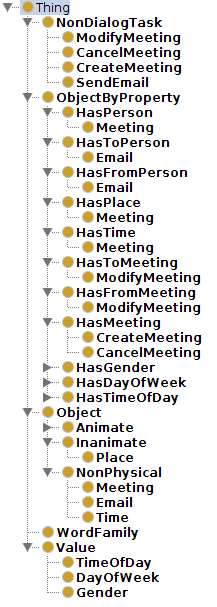
\includegraphics[width=150px]{sample-ontology-screenshot}
  \caption{YODA sample domain ontology}
  \label{sample-ontology-figure}
\end{figure}

Figure \ref{sample-ontology-figure} shows the class hierarchy for the domain ontology.

\section {Define the Dialog Functionality} \label{dialog-management-section}

\subsection {Dialog Tasks}
The developer defines what dialog tasks

\subsection {Non-dialog Tasks}
Several aspects of a non-dialog task will effect how the dialog manager interacts with them.
In addition to implementing the execution of these tasks, the developer must define the information relevant for dialog management.


\begin{figure}[ht*]
\centering
\rule{\textwidth}{1pt}
\small
\begin{minted}[linenos=true]{java}
public class NonDialogTaskPreferences {
    // if explicit confirmation is always required before the 
    // task is executed, set alwaysRequireConfirmation to true
    public boolean alwaysRequireConfirmation;

    // all the rewards and penalties are given as positive 
    // numbers, penalties are converted to negative numbers for
    // decision-making
    public double penaltyForDelay;
    public double rewardForCorrectExecution;
    public double penaltyForIncorrectExecution;

    // define the slots that are required to be defined by the
    // user before execution is possible
    public Set<String> slotsRequired;

    public NonDialogTaskPreferences(
        boolean alwaysRequireConfirmation, 
        double penaltyForDelay, 
        double rewardForCorrectExecution, 
        double penaltyForIncorrectExecution, 
        Set<String> slotsRequired) {
        this.alwaysRequireConfirmation = 
            alwaysRequireConfirmation;
        this.penaltyForDelay = penaltyForDelay;
        this.rewardForCorrectExecution = 
            rewardForCorrectExecution;
        this.penaltyForIncorrectExecution = 
            penaltyForIncorrectExecution;
        this.slotsRequired = slotsRequired;
    }
}
\end{minted}
\rule{\textwidth}{1pt}
\caption{The NonDialogTask interface}
\label{NonDialogTaskPreferences-code-figure}
\end{figure}

Figure \ref{NonDialogTaskPreferences-code-figure} shows the definition for the NonDialogTaskPreferences class.
It contains several parameters which determine the reward and penalty (negative reward) received by the system for executing a task, delaying execution of a task, and incorrectly executing a task or executing a task with incorrect parameters.
These preferences are used by the dialog manager to perform decision-theoretic dialog management, and may be used to train reinforcement-learning dialog managers in the future.

There is another parameter, alwaysRequireConfirmation, that can be set to true if the dialog manager is required to get a confirmation from the user before performing an non-dialog task.
Depending on the cost / benefit tradeoff, the dialog manager may decide to request a confirmation before executing a non-dialog task even if the flag is not set, and setting a high penalty for incorrect execution can make explicit confirmation requests more likely, but setting the flag allows the designer to enforce strict transparency.

In our Figure \ref{SendEmailTask-code-figure} line 5-7, we show the preferences declaration for the send-email task.
Here, we set alwaysRequireConfirmation to true, so the user will always be asked for explicit confirmation before an email is sent, as in the following example:

\begin{alltt}
\textbf{User} Send an email to Jerry.
\textbf{System} You want me to send an email to Jerry, right?
\textbf{User} Yes.
\textbf{System} Ok.
\textbf{System} <executes task>
\end{alltt}

In our Figure \ref{CreateMeetingTask-code-figure} line 5-10, we show the preferences declaration for the create-meeting task.
Here, we set alwaysRequireConfirmation to false, so the system is allowed to perform the task without an explicit confirmation, as in the following example:

\begin{alltt}
\textbf{User} Set up a meeting this afternoon with Jerry in my office.
\textbf{System} Ok.
\textbf{System} <executes task>
\end{alltt}

The last parameter of the NonDialogTaskPreferences class sets requirements for what must be specified for a task to be executable.
As is shown in the preference declarations from Figures \ref{SendEmailTask-code-figure} and \ref{CreateMeetingTask-code-figure}, sending an email only requires a sender, while creating a meeting requires a description of a meeting with at least one time, place, and attendee.
The dialog manager will not consider executing a task until all its required slots are filled, and will instead engage in slot-filling dialog, as in the following example:

\begin{alltt}
\textbf{User} Set up a meeting this afternoon.
\textbf{System} Where will this meeting be?
\textbf{User} In my office.
\textbf{System} Who is this meeting with?
\textbf{User} Jerry.
\textbf{System} Ok.
\textbf{System} <executes task>
\end{alltt}


After basic preferences have been defined, the NonDialogTask interface, shown in figure \ref{NonDialogTask-interface-code-figure}, must be implemented for each non-dialog task.
Two implementations of this are shown in this tutorial, SendEmailTask is shown in figure \ref{SendEmailTask-code-figure}, and CreateMeetingTask is shown in figure \ref{CreateMeetingTask-code-figure}

\begin{figure}[ht*]
\centering
\rule{\textwidth}{1pt}
\small
\begin{minted}[linenos=true]{java}
public interface NonDialogTask {

    public enum TaskStatus {SUCCESSFULLY_COMPLETED, 
      CURRENTLY_EXECUTING_BLOCKING,
      CURRENTLY_EXECUTING_NOT_BLOCKING, FAILED}

    // return preferences object
    public NonDialogTaskPreferences getPreferences();

    // the probability that the taskSpec can be executed (0-1)
    public double assessExecutability(SemanticsModel taskSpec);

    // return the string ID of the executing task (taskID)
    public String execute(SemanticsModel taskSpec);

    // return the string status indicator for the taskID
    public TaskStatus status(String taskID);

}
\end{minted}
\rule{\textwidth}{1pt}
\caption{The NonDialogTask interface}
\label{NonDialogTask-interface-code-figure}
\end{figure}


The assessExecutability method is a task-specific method for informing the dialog manager how likely it is a task will succeed.
For example, sending an email may be guarenteed to fail if the device does not have working internet.
For situated agents such as robots, there is always some non-negligible chance that an attempted physical action will fail.
The dialog manager will incorporate these probabilities into its decision-making process.
Intuitively, it will hesitate to perform actions which are likely to fail, and eagerly execute actions which are likely to succeed.

The execute method executes the actual task.
This will call developer-defined functions and libraries to actually send emails, reserve meeting rooms, etc.

The status method checks a task's status, which can be one of the following:
\begin{itemize}
\item SUCCESSFULLY\_COMPLETED
\item CURRENTLY\_EXECUTING\_BLOCKING
\item CURRENTLY\_EXECUTING\_NOT\_BLOCKING
\item FAILED
\end{itemize}

When a task is blocking, the dialog system is temporarily de-activated.
In this tutorial, we assume that a separate module is called for email dication, so the send-email task is blocking.

\begin{figure}[ht*]
\centering
\rule{\textwidth}{1pt}
\small
\begin{minted}[linenos=true]{java}
public class SendEmailTask implements NonDialogTask {
    private static Integer instanceCounter = 0;
    private static Map<String, TaskStatus> executionStatus = 
        new HashMap<>();
    private static NonDialogTaskPreferences preferences = 
        new NonDialogTaskPreferences(true, 1, 20, 20,
            new HashSet<>(Arrays.asList("hasToPerson")));

    @Override
    public NonDialogTaskPreferences getPreferences() {
        return preferences;
    }

    @Override
    public double assessExecutability(SemanticsModel taskSpec) {
        // this works because assessExecutability is never
        // called unless all the required slots are present
        return 1.0;
    }

    @Override
    public String execute(SemanticsModel taskSpec) {
        System.out.println("Executing task: send email");
        System.out.println(taskSpec);
        String ans = "SendEmailTask:"+instanceCounter.
            toString();
        instanceCounter += 1;
        // There is no real implementation, so we just set 
        // the status to successfully completed
        executionStatus.put(ans,
            TaskStatus.SUCCESSFULLY_COMPLETED);

        /*
         * In the envisioned implementation, a separate
         * dictation program would run while the other 
         * program is run, the dialog manager should block, as
         * in the following commented lines
         */
        // executionStatus.put(ans,
        //    TaskStatus.CURRENTLY_EXECUTING_BLOCKING);
        // dictationProgram.run();

        System.out.println("taskID: "+ans);
        return ans;
    }

    @Override
    public TaskStatus status(String taskID) {
        return executionStatus.get(taskID);
    }
}
\end{minted}
\rule{\textwidth}{1pt}
\caption{The SendEmailTask implementation}
\label{SendEmailTask-code-figure}
\end{figure}





\begin{figure}[ht*]
\centering
\rule{\textwidth}{1pt}
\small
\begin{minted}[linenos=true]{java}
public class CreateMeetingTask implements NonDialogTask {
    private static Integer instanceCounter = 0;
    private static Map<String, TaskStatus> executionStatus = 
        new HashMap<>();
    private static NonDialogTaskPreferences preferences =
            new NonDialogTaskPreferences(false, 1, 20, 15,
                    new HashSet<>(Arrays.asList(
                        "hasMeeting.hasTime", 
                        "hasMeeting.hasPlace", 
                        "hasMeeting.hasPerson")));

    @Override
    public NonDialogTaskPreferences getPreferences() {
        return preferences;
    }

    @Override
    public double assessExecutability(SemanticsModel taskSpec) {
        return 1.0;
    }

    @Override
    public String execute(SemanticsModel taskSpec) {
        System.out.println("Executing task: create meeting");
        System.out.println(taskSpec);
        String ans = "CreateMeetingTask:"+instanceCounter.
            toString();
        instanceCounter += 1;
        // There is no real implementation, so we just set the
        // status to successfully completed
        executionStatus.put(ans, 
            TaskStatus.SUCCESSFULLY_COMPLETED);
        System.out.println("taskID: "+ans);
        return ans;
    }

    @Override
    public TaskStatus status(String taskID) {
        return executionStatus.get(taskID);
    }
}
\end{minted}
\rule{\textwidth}{1pt}
\caption{The SendEmailTask implementation}
\label{CreateMeetingTask-code-figure}
\end{figure}










%% \section {Define interfaces to External Databases}
%% Classes in the ontology correspond to supporting databases.

%% There are two types of supporting databases, corresponding to two primary functions:
%% \begin{itemize}
%% \item{\textbf{Long-term Memory Database:}Store objects from interactions in long-term memory to keep reasoning in working memory tractable while allowing for possible retrieval at a later date}
%% \item{\textbf{Reference Database:} Store and index a large collection of reference objects (the standard use paradigm of a database)}
%% \end{itemize}

%% By default, every class defined in the ontology has no supporting reference database, and an independent long-term memory database.
%% If the developer wants to provide a reference database they may do so.
%% The developer can decide weather or not the dialog system is allowed to insert to that database.
%% If the dialog system is not allowed to insert, then a separate long-term memory database will be automatically created.
%% Otherwise, the reference database will provide both long-term memory and reference functions.

%% Reference databases must be Sesame RDF databases.
%% Many existing databases are in relational format and are accessed via SQL.
%% These databases can be represented as RDF databases, as is described in \href{http://www.w3.org/2005/Incubator/rdb2rdf/RDB2RDF_SurveyReport.pdf}{A Survey of Current Approaches to Mapping of Relational Databases to RDF}.
%% YODA requires a map between slots and properties which are shared by the domain ontology and the database schema.
%% YODA only allows a one-to-one mapping of properties and slots, but allows certain properties to exist only in the reference database.

%% Any database interface that does not have the default setting is defined by modifying the yoda/interfaces/DatabaseInterfaces.java file.




%% \section {Build a lexicon for NLG}
%% Initial linguistic information should be associated with each new class and instance.
%% The two figures below show examples of the linguistic information associated with the objects specified above.
%% The complete example is given in the attached owl file.

%% The program TestLexicalEntry.java generates sample sentences based on the lexicon provided by the developer.
%% The developer can use this program to test that their lexicon generates sensible sentences and covers the full variety of things the developer expects to be said about the object.
%% Call it from the command line using: java TestLexicalEntry.java -e [entryID]


%% \section {Train SLU and speech modules with artificial data}

%% To build an initial SLU component, YODA takes the generated lexicon and creates a large training set.
%% It adds artificial noise to the training set for robustness, and extends the training set using wordnet synonyms.
%% It then trains a state-of-the-art SLU component based on this artificial data.

%% To build an initial SLU component, run java GenerateInitialSLUComponent.java .
%% Include -v in the command line arguments after the filename to see cross-validation results within the auto-generated corpus.

%% The training data set is retained in yoda/SLU/artificial\_train.txt, and the domain-specific annotation scheme is described in yoda/SLU/annotation\_scheme.txt .
%% As real data is collected, the SLU component can be improved by incorporating annotated real-world examples.

%% To build an improved SLU component, put labeled real-world data in yoda/SLU/real\_data.txt in the same format as artificial\_rain.txt, then run: java GenerateImprovedSLUComponent.java .
%% Include a -v in the arguments after the filename to see validation results and a comparison between the initial and the improved systems.

%% It will likely be the case that as real data is collected, the developer will discover that the domain and lexicon definitions should be extended to improve coverage of users actully say.
%% We recommend that this be done by extending the ontology rather than simply training the improved model.
%% The purpose of the improved model is to improve the component's likelihood model for different utterances, not to compensate for poor coverage.

%% To generate a language model based on the automatically generated sentences and the real data examples, run the script build\_language\_model.sh .


%% \section {Build sensor interfaces}
%% YODA dialog systems support situated interaction by defining sensor interfaces.
%% Sensors can report the existance of new entities, and their properties and relations.
%% The interfaces define a message protocol used to receive updates from the sensors.

%% Some of the information provided in the protocol includes:
%% \begin{itemize}
%% \item Expected framerate
%% \item Expected consistency of the sensor readings over time
%% \item Type of confidence markup (N-best, Bayes net, full CPT)
%% \item Overlap interface (Define the overlap between this sensor and other sensors)
%% \item Relevance interface (Choose a strategy for defining how relevance to the ongoing discourse should be tracked for objects in this sensor stream)
%% \item Expected recall of objects (effects dialog strategy)
%% \item Expected precision (of some slot?)
%% \end{itemize}

%% \subsection {Sensor belief tracking in Yoda}
%% YODA designers will explore belief-tracking and sensor fusion approaches that generalize to dynamic situated domains.

%% \subsection {Long-term Memory and Discourse Relevance in YODA}
%% YODA designers will explore different strategies for tracking objects' relevance to an ongoing discourse, and for using that relevance to move information between long-term and working memory.
%% The different properties of different sensor types will be better suited for different relevance strategies.

\bibliographystyle{acm}
\bibliography{/home/cohend/Dropbox/Documents/bibtex_db}

\end{document}
